\documentclass[conference]{IEEEtran}
\usepackage{cite}
\usepackage{tcucosc}
\usepackage{lipsum}
\usepackage{graphicx}


\title{Parallelized Traffic Simulation in C++}

\author{
\IEEEauthorblockN{Zach Alaniz}
\IEEEauthorblockA{Department of Computer Science\\
College of Science and Engineering\\
Texas Christian University\\
Fort Worth, Texas 76129\\
Email: z.a.alaniz@tcu.edu\\}
\and
\IEEEauthorblockN{Saby Sahoo}
\IEEEauthorblockA{Department of Computer Science\\
College of Science and Engineering\\
Texas Christian University\\
Fort Worth, Texas 76129\\
Email: s.sahoo@tcu.edu\\}
\and
\IEEEauthorblockN{Bradley Schoeneweis}
\IEEEauthorblockA{Department of Computer Science\\
College of Science and Engineering\\
Texas Christian University\\
Fort Worth, Texas 76129\\
Email: b.schoeneweis@tcu.edu\\}
}



\begin{document}


\maketitle


\begin{abstract}
This semester research project investigates the potential speedups and scalability of running a traffic simulation in parallel using C++ and OpenMP. These speedups are evaluated by comparing the sequential performance to the parallel performance when varying thread counts for a fixed-size, randomized input. While a large percentage of the program is inherently sequential due to computation, the process of transitioning from one state to another was parallelized. 
\end{abstract}
\bigskip
\begin{IEEEkeywords}
OpenMP, Cellular Automata, Parallel Simulation, C++
\end{IEEEkeywords}

\section{Introduction}
Extensive research and improvement has been made over the years in the field of study that is parallel computing. Falling within this domain of study is the topic of simulation, and more specifically, traffic simulation. The ability to optimize light scheduling and move cars from one point to another in an efficient, organized manner is paramount to day-to-day travel. Being able to apply parallel computing to simulate increasingly large traffic environments leads to many interesting research topics and advances in road safety, traffic capacity, economic impact, among many others. The topic of simulating traffic flow for increasingly large sizes of roads is the topic of interest in the following research. Real life traffic flow allows for movement when possible at all times, and by utilizing parallel computing topics and tools, the speedup of a traffic simulation should prove beneficial in seeing how a particular road and intersection works for an increasingly large amount of cars funneling in and out.  \\
\hspace*{.2cm} Traffic simulation naturally lends itself to parallel ideas. Decomposing the movement of cars into a sub-domain of problems and updating traffic flow in parallel, just as normal traffic would run, is one method to improved performance. Thus, a parallel solution to traffic flow needs to be able to parallelize any movement and update that could be happening concurrently. The dynamic nature of traffic also plays a large role in this type of simulation, but was handled to leave a larger emphasis on the updating of car movements. The following research being presented simulates traffic flow through a four-way stop, which includes two-lane roads from all directions. The simulation was built with C++ utilizing a cellular automaton approach, and parallel integration was made with OpenMP, an application programming interface (API) that supports shared memory multiprocessing. The following is an overview of the remainder of the paper: Background research on every tool and idea used as well as reasons for why they were chosen, sequential solution and design, parallel integration and results, and finally a summary with conclusions of our research.

\section{Background and Related Research}
%%%%%%%%%\lipsum[2] \cite{Laszlo1996}
Chances are if you have rode in a vehicle, you have come across a four-way stop being controlled by traffic lights. A four-way traffic stop has roads leading from all four directions (north, east, south, west) where each direction takes a turn moving towards its destination as directed by the controlling traffic light. The traffic light operates in three states: red, green, and yellow, where green means go, red means stop, and yellow means slow down. Assuming each direction is at least a two-lane road, any car driving on the outer most lane is capable of taking a right turn at the traffic light intersection if oncoming traffic is clear, regardless of the state of the light. Cars in the innermost lanes are also capable of making a left turn, given that their light is currently green. The light itself cycles on a timer allowing for each lane to have its own turn to proceed, which creates the flow of traffic. This four-way model is what our simulation is derived from, which will be explained in a later section. \\
\hspace*{.2cm} The placement of cars along any road is relatable to a data model studied in computer science and related fields known as \textit{cellular automata}. Formally, cellular automota is defined as a collection of cells on a grid that evolves during a number discrete time steps according to a set of rules based on the states of neighboring cells. The rules are then applied iteratively for as many time steps as desired [1]. Cellular automata has been studied since the early 1950s and started as a model for biological systems. The grid and state like approach of cellular automata was taken and applied to our simulation too represent state of traffic flow and position of cars within a street.

\section{Serialization Technique}
To design our serial solution to the four-way traffic simulation, we began by deciding on using an array type data structure to represent each lane and store car states. Since our simulation runs with four horizontal lanes handling cars moving east and west, and four vertical lanes handling cars moving north and south, our solution uses eight arrays in total to hold all data. An array data structure was chosen for a few reasons. The first being because C++ arrays store memory contiguously, meaning the data is laid out next to each other with no gaps in between. This type of memory layout is ideal because it makes data parallelization simple, as well as allows for use of the cellular automata model. Data layout was the main reason that moved the design away from an object-oriented approach. Storing objects in C++ leads to offsets between data in memory, making it much harder to parallelize when the time comes. Within each of the eight arrays (roads) holds a variable number of cars represented by and integer value from $0, 1, 2, $ or $3$ that each correspond to a specific action within the simulation. Each integer is defined as follows:\\ 

\begin{itemize}
	\item 0: Empty
	\item 1: Car moving straight
	\item 2: Car taking a right
	\item 3: Car taking a left \\
\end{itemize}

The eight roads included in the traffic simulation also leads to a $4x4$ intersection point holding 16 cells. This intersection point represents the cars that are moving to the other side of the road. To keep track of these cars we split the work between horizontal and vertical, where either of the horizontal and vertical arrays can be holding cars within the intersection at any state. \\
The last important aspect of designing the simulation was how to handle light timing for every direction. To have our light timing continuously looping a rotating array was used that shifted a single value to the right on a timer, which moved the state of one light on to the next. This way the light timing would continuously run until the simulations end.\\
\hspace*{.2cm} Two different approaches were used as input to populate our roads for simulation. The first was input by csv, where the csv was filled with numbers representing cars and could be read in to populate road data. This input was useful when testing on smaller inputs and at the beginning of logic development, because it allows for controlled traffic states and expected output. The next type was randomized input. A command line argument is used to gather the dimensions of fo each road size and corresponding car types are randomly placed at every spot within each road based off of probability. This version of input allowed for increasingly large input sizes to be created and tested for more extensive testing once logic development was completed. \\
\hspace*{.2cm} To confirm correctness of development, an important output function was also created. The main version of output, which cleanly represents a traffic simulation, was done using UTF-8 characters to represent lights and prints to the console showing an overhead view of traffic current traffic. At any time this output only represents the middle $20x20$ view of the traffic, including the $4x4$ intersection. This output leads to a minimum road size of 20 and allows for an easy view of the simulation regardless of the input size. To go along with this, important current road statistics are also shown to know when the simulation will be ending, such as car's exited, and how long each run of the simulation is taking.  \\
\hspace*{.2cm} The updating of car positions is where cellular automata comes in. Each car is moved to its next state in the simulation by shifting them to the next spot in the array. This array shifting is done by indexing, which will prove to be of interest and explained later on. Before proceeding, each car must check ahead of them in the direction they are moving for an empty cell, which is in line with the model of cellular automata. Throughout the simulation cars are continuously checking states before moving through each cell until the simulation is complete. \\
\hspace*{.2cm}  The simulation is run state by state until every car has exited. As the state simulation begins, each state is done one time followed by a short sleep time before the next states run. To run the simulation, there is a pre-set sleep time that allows for state by state printing to the console between each step in the simulation, which can also be lowered to run a faster simulation. This set sleep time also controls the time each green light is set for, called light time, to scale it according to the speed and size of the simulation. Lastly there is a clear time, which serves as the simulations yellow light, and allows for cars within the intersection to clear out before the next light becomes green. Green and yellow lights are calculated in the following way: \\

Light time $= sleep time \cdot factor$ \\

Clear time $= sleep time \cdot 4$ \\

where $factor$ is scaled to the size of the simulation. Clear time is always set to 4 because the intersection size is constant.

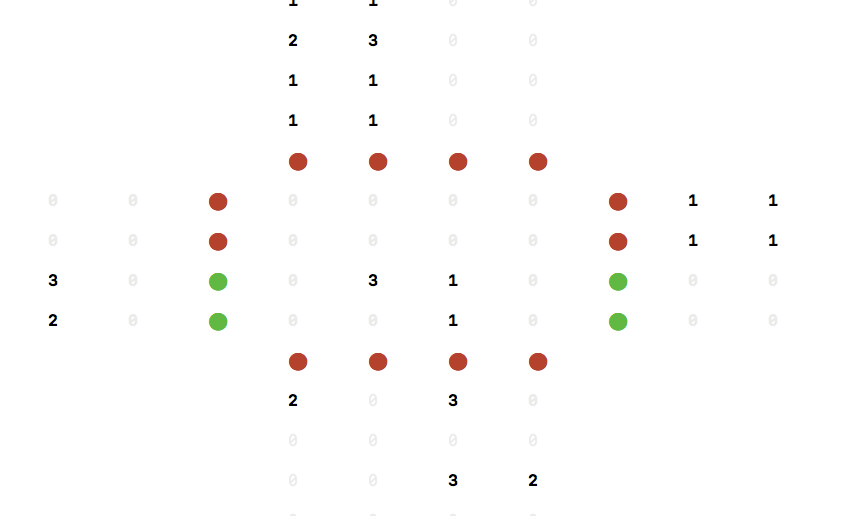
\includegraphics[width=0.5\textwidth]{green}




\section{Parallelization Technique}
\lipsum[3] \cite{ORourke2005}

\section{Summary of Results}
\lipsum[4]

\section{Conclusions, Lessons Learned, and Future Work}
\lipsum[5]

\bibliographystyle{ieeetr}
\bibliography{HPC_Project}

\end{document}